\documentclass{article}
\usepackage[utf8]{inputenc}
\usepackage{amsmath,amssymb,amsfonts}
\usepackage{amsthm}
\let\oldAA\AA
\renewcommand{\AA}{\text{\normalfont\oldAA}}
\usepackage[makeroom]{cancel}
\usepackage{graphicx}
\usepackage{caption}{\tiny }
\usepackage[affil-it]{authblk}
\usepackage{multirow}
\usepackage[table,xcdraw]{xcolor}
\usepackage{titlesec}
\usepackage{longtable}
\usepackage{wrapfig}
\usepackage{mathtools}
\usepackage{bm}
\usepackage{esvect}
\usepackage[colorlinks = true,
            linkcolor = blue,
            urlcolor  = blue,
            citecolor = blue,
            anchorcolor = blue]{hyperref}

\newcommand{\MYhref}[3][blue]{\href{#2}{\color{#1}{#3}}}%
\usepackage[
bookmarksopen,
bookmarksdepth=2,
breaklinks=true
]{hyperref}
\usepackage{arxiv}
\usepackage[utf8]{inputenc} % allow utf-8 input
\usepackage[T1]{fontenc}    % use 8-bit T1 fonts
\usepackage{hyperref}       % hyperlinks
\usepackage{url}            % simple URL typesetting
\usepackage{booktabs}       % professional-quality tables
\usepackage{amsfonts}       % blackboard math symbols
\usepackage{nicefrac}       % compact symbols for 1/2, etc.
\usepackage{microtype}      % microtypography
\usepackage{lipsum}		% Can be removed after putting your text content
\usepackage{graphicx}
\usepackage{natbib}
\usepackage{doi}
\renewcommand\refname{Kaynakça}



\title{Müon Çarpıştırıcıları ve Fizik Potansiyeli}

%\date{September 9, 1985}	% Here you can change the date presented in the paper title
%\date{} 					% Or removing it

\author{ \href{https://orcid.org/0000-0002-1684-9602}{\includegraphics[scale=0.06]{orcid.pdf}\hspace{1mm}Halil Kolatan} \\
	Ankara Üniversitesi\\
	Fen Fakültesi 
	Fizik Bölümü }\\
% Uncomment to remove the date

\date{23 Haziran 2021}

% Uncomment to override  the `A preprint' in the header
%\renewcommand{\headeright}{Technical Report}
%\renewcommand{\undertitle}{Technical Report}
%\renewcommand{\shorttitle}{\textit{arXiv} Template}

%%% Add PDF metadata to help others organize their library
%%% Once the PDF is generated, you can check the metadata with
%%% $ pdfinfo template.pdf
\hypersetup{
pdfauthor=Halil Kolatan}

\begin{document}
\maketitle


\begin{abstract}
Yüksek enerjili parçacık çarpıştırıcıları, parçacık fiziğinin doğasını anlamak için vazgeçilmez bir araçtır. Yeni fizik arayışımızla birlikte mevcut çarpıştırıcıları da geliştirmek zorundayız. Birçok yeni çarpıştırıcı seçeneklerinden biri müon çarpıştırıcılarıdır. Müon çarpıştırıcıları, yüksek enerji fiziği için büyük bir potansiyele sahiptir. Müon çarpıştırıcıları çok yüksek enerjilerde nokta benzeri parçacıkların çarpışmalarını bize sunabilir ve diğer lepton çarpıştırıcıların enerji sınırını güçlü bir şekilde aşabilir. Bununla birlikte, müon çarpıştırıcıları tasarlayabilmek için birçok teknik sorun da mevcuttur. Bu araştırma ödevi müon çarpıştırıcılarını, tasarımlarını ve yeni fizik potansiyelini incelemektedir.
\end{abstract}

%keywords can be removed
%\keywords{Müon çarpıştırıcısı \and Second keyword \and More}


\section{Giriş}

 Parçacık fiziğinde keşif arayışı her zaman mümkün olan en yüksek enerjilerde deneyler gerektirmiştir. Yüksek enerjili parçacık çarpıştırıcıları ise şimdiye kadar parçacık fiziğinin doğasını anlamak için vazgeçilmez bir araç olmuştur. Parçacık demetlerini çok yüksek enerjiyle hızlandırmak, bu demetleri çarpıştırmak ve bu çarpışmaların oluşturduğu parçacıkları tespit etmek için yeni teknikler geliştirilmiştir. Higgs bozonunun başarılı keşfi ve LHC'de (Büyük Hadron Çarpıştırıcı) yeni parçacıklar ve kuvvetler arayışı bu geleneğe dayanmaktadır. Standart Modelin (SM) ötesinde, yükseltilmiş bir enerji seviyesinde yeni parçacıklar arayışını sürdürebilecek bir tesis yaratmak için teknikte daha fazla ilerleme gereklidir. Böyle bir tesisin, yeni fiziği hem doğrudan hem de dolaylı olarak keşfetmek için, birkaç TeV'i aşan kütle merkezi enerjilerinde çarpışmalar sağlaması ve çarpışma ürünlerini hassas bir şekilde ölçebilmesi gerekecektir. Bu özellikler, olası LHC veya HL-LHC keşiflerini karakterize etmek için de gerekli olacaktır. Leptonların temel doğası, lepton-antilepton çarpıştırıcılarını enerji sınırında hizmet etmek için ideal bir çarpıştırıcı yapar [1].
 
  \begin{figure}[h]
 \centering
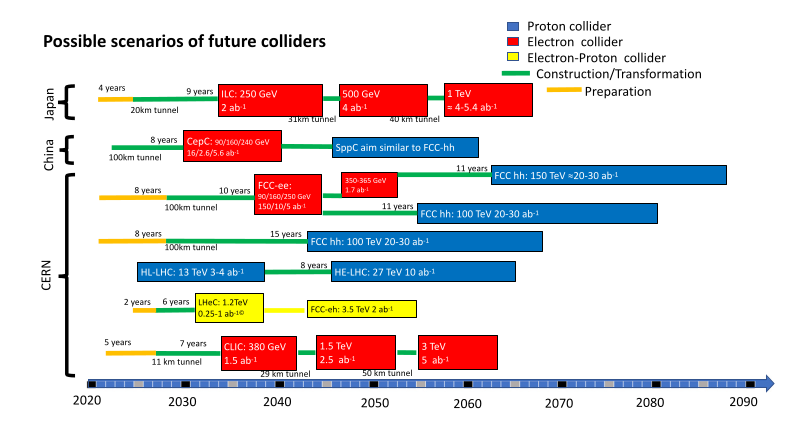
\includegraphics[width=14cm]{image/Ekran Görüntüsü - 2021-06-23 10-37-41.png}
\caption*{Şekil 1. Hazırlık (turuncu), inşaat (yeşil) halindeki gelecek çarpıştırıcılar ve veri alma için gereken zamanı gösteren potansiyel zaman çizelgeleri [4].}
	\end{figure}

 
 \section{Müon Çarpıştırıcıları}
 
 Müon çarpıştırıcıları fikri ilk olarak Skrin ve Neuffer tarafından ortaya atıldı. Mevcut şemaya daha çok benzeyen bir şemayı ilk olarak Neuffer ve Palmer sundu ve o zamandan beri sürekli olarak artan ayrıntılarla incelendi. Müon çarpıştırıcıları, çoklu-TeV enerji aralığında büyük keşif potansiyeli sunar. Elektrondan 207 kat daha ağır olan müon, aynı enerjiye sahip elektron ışınlarına kıyasla sinkrotron radyasyonunu 10$^{9}$ kat bastırır. Bu nedenle halkalar, müon ışınlarını verimli bir şekilde hızlandırmak ve onları tekrar tekrar çarpıştırmak için kullanılabilir. Ayrıca müon çarpıştırıcısı birden fazla deneye hizmet edebilir [1,2].
 
 Bugün, elektron-pozitron çarpıştırıcıları için gelişmiş seçenekler mevcuttur: CERN'deki Future Circular Collider (FCC) ve Compact Linear Collider (CLIC) planları (bk. Şekil 1 ve 2); Japonya'daki International Linear Collider (ILC) ve Çin'deki Circular Electron-Positron Collider (CEPC). FCC, gerekli kütle merkezi enerjilerinde çok yüksek ışınlık sunar. Bununla birlikte, ulaşılabilecek maksimum enerji, çarpıştırıcı halkasında sinkrotron emisyonu ile sınırlıdır ve 100 km'lik dairesel hızlandırıcı için 365 GeV'lik bir kütle merkezi enerjisine karşılık gelir. Doğrusal çarpıştırıcılar, parçacıkları sinkrotron radyasyonu yaymadan hızlandırır ve bu nedenle daha yüksek enerjilere ulaşabilir. ILC başlangıçta 250 GeV'de çalışacak ve 1 TeV'e kadar ulaşabilecekken CLIC 3 TeV'e ulaşacak şekilde tasarlandı. Bununla birlikte, doğrusal bir çarpıştırıcı ile daha yüksek enerjilere çıkabilmek için aşılması gereken iki temel problem vardır: Birincisi, demetlerin tek bir lineer hızlandırıcıda tam enerjiye hızlandırılması gerekmektedir; ikincisi, tek bir çarpışmada sadece bir kez kullanılabilir. Daha yüksek enerjilerde lineer hızlandırıcı daha uzun olmalıdır ve bu nedenle daha maliyetlidir, demetin tek çarpışmada kullanılması da makul bir güç tüketimi için elde edilebilen ışınlılığı sınırlar [3].
 
 \begin{figure}[h]
 \centering
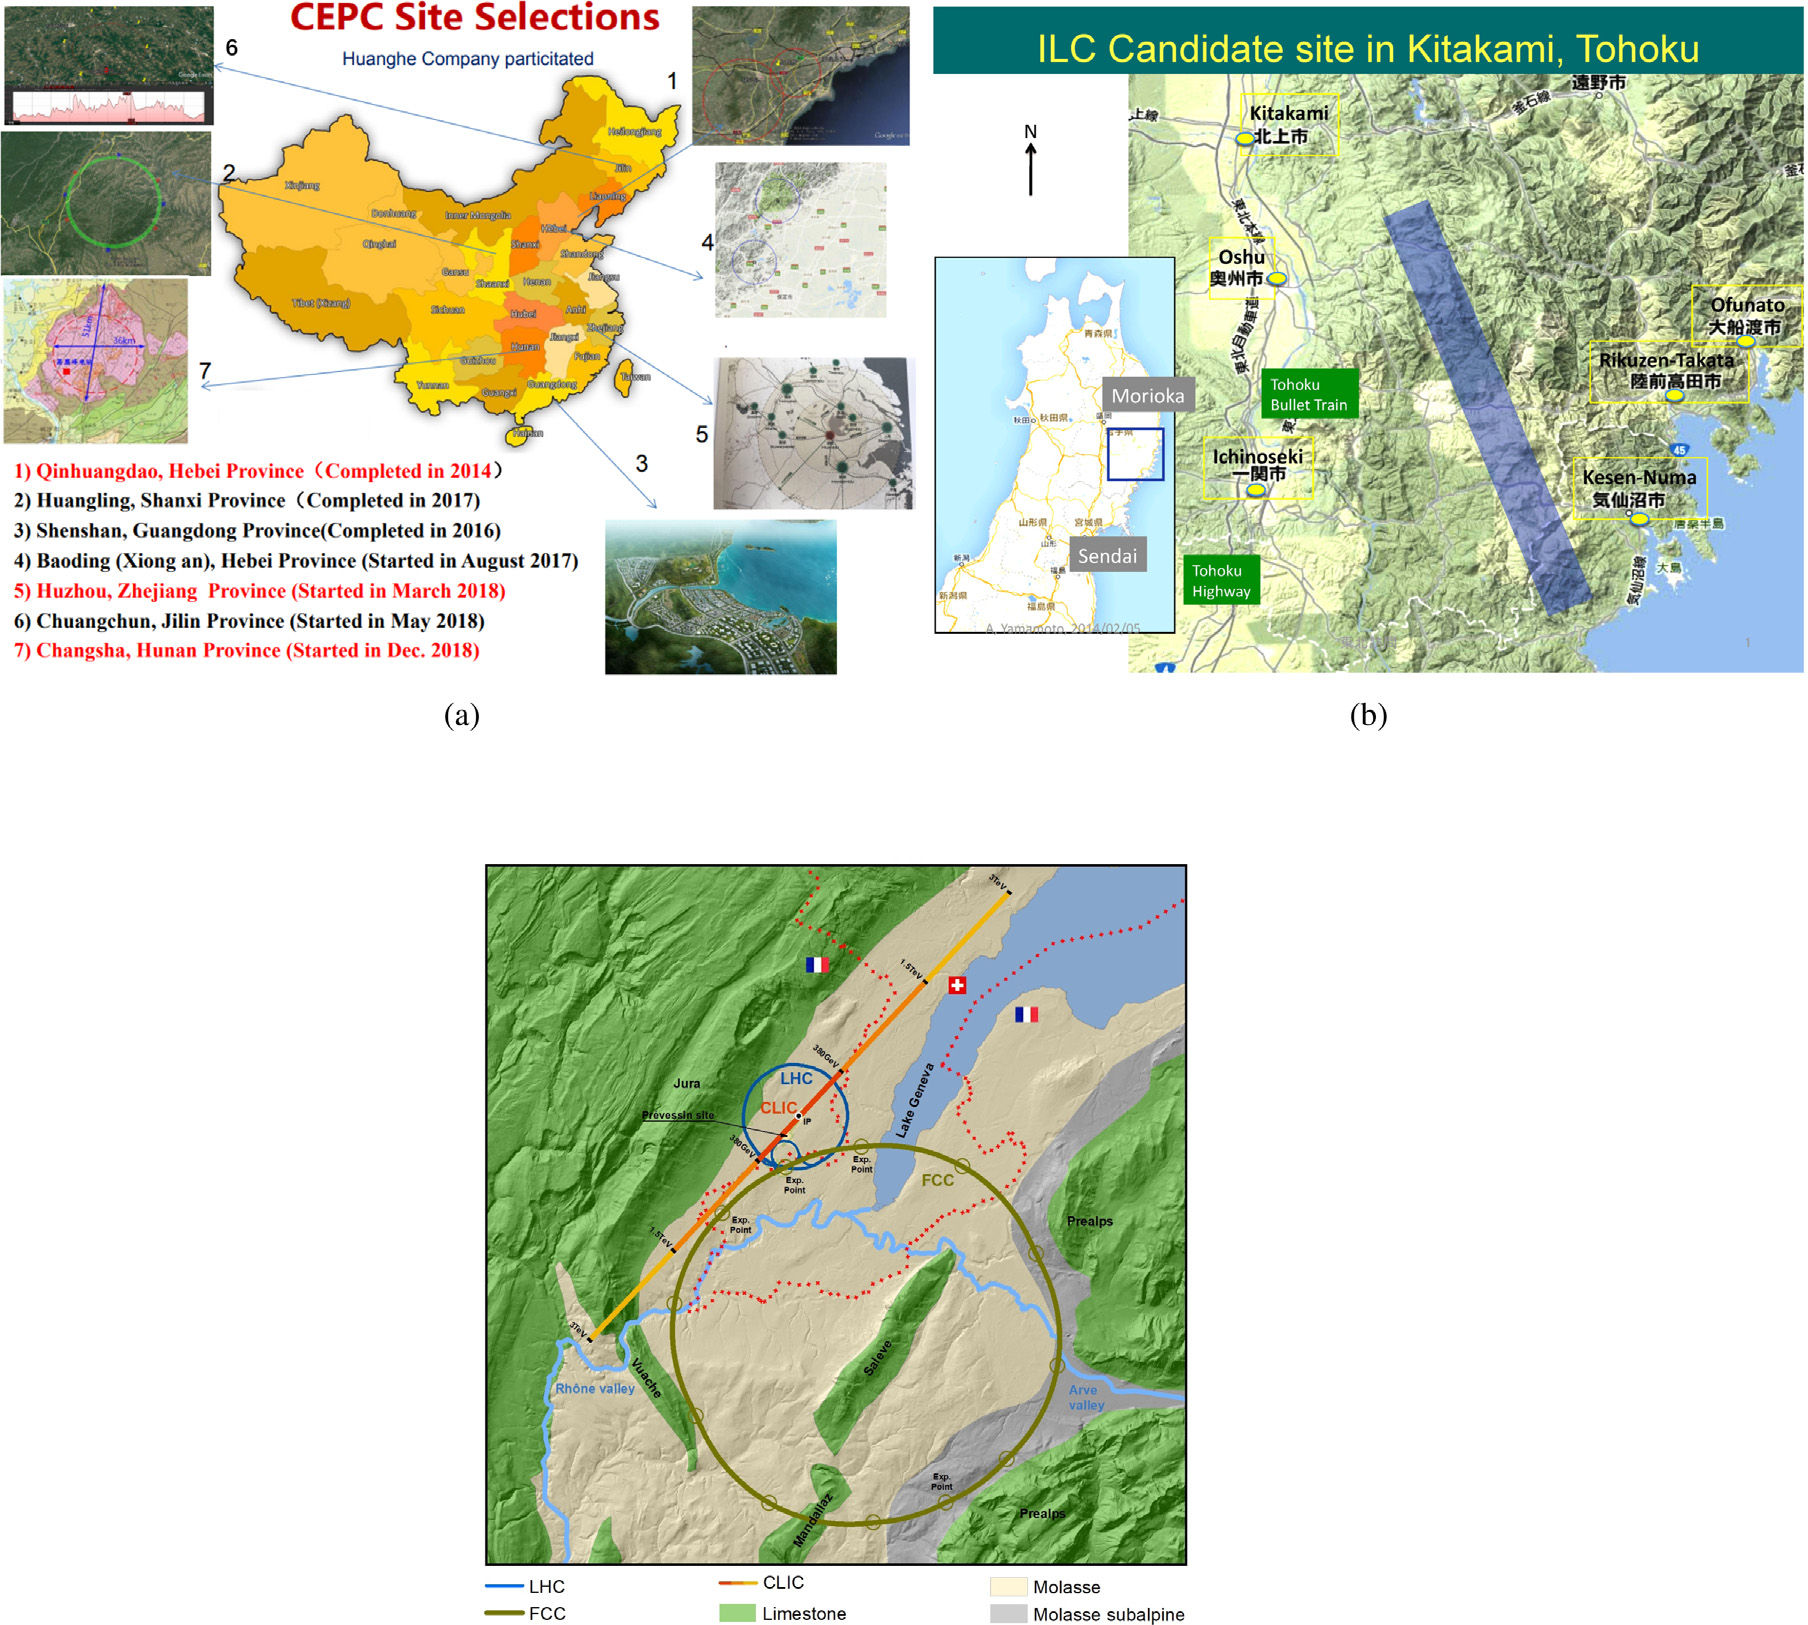
\includegraphics[width=11cm]{image/1111.png}
\caption*{Şekil 2. (a) CEPC ve SppC, (b) ILC ve (c) CLIC ve FCC için potansiyel bölgeler ve planları [4].}
	\end{figure}

 
 
Bu sorunların üstesinden gelmek için dahiyane bir çözüm, elektronları ve pozitronları müonlar ve anti-müonlarla değiştirmektir. Bir müon çarpıştırıcısı hem hassas hem de güçlü bir keşif çarpıştırıcısı olacaktır, çünkü çok yüksek enerjilerde, diğer lepton çarpıştırıcılarının enerji erişimini aşan nokta benzeri parçacıkların çarpışmalarını bize sunabilir. Müonlar, protonların aksine temel parçacıklardır ve bu yüzden istediğimiz efektif enerjiye ulaşabiliriz. Ayrıca özel bir müon çarpıştırıcısı, Higgs rezonansını tarayabilen ve kütlesini hassas bir şekilde ölçebilen tek lepton-antilepton çarpıştırıcı seçeneğidir. Bu nedenle bir müon çarpıştırıcısı, hem hassas bir çarpıştırıcı hem de bir keşif makinesi olarak yeni fizik aramak ve dar rezonansları çözmek için idealdir [1,3].

\subsection{Avantajları}

Müon çarpıştırıcılarının, başlıca avantajları şunlardır [2]: 

\begin{itemize}
    \item Yüksek enerjili elektron çarpıştırıcılarının doğrusal ve uzun olmasını gerektiren sinkrotron radyasyonu,müon çarpıştırıcısında bastırıldığı için Şekil 3'de görüldüğü üzere dairesel ve daha küçük olabilir. Şekil 2 ile kıyasladığımızda ise müon çarpıştırıcısının ne kadar efektif olabileceğini görebiliyoruz.
\end{itemize}

 \begin{figure}[h]
 \centering
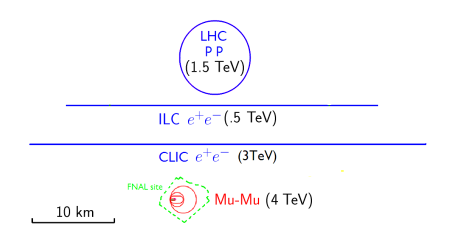
\includegraphics[width=11cm]{image/Ekran Görüntüsü - 2021-06-23 02-34-03.png}
\caption*{Şekil 3. Çarpıştırıcıların göreli boyutları ve etkin kütle merkezi enerjileri [2].}
	\end{figure}
	
	
\begin{itemize}
    \item Çarpıştırıcının halkası dairesel olduğundan, müon demetleri birçok kez çarpışır. Bu da daha çok veri toplama imkanı sağlamaktadır.
\end{itemize}

\begin{itemize}
    \item Çarpıştırıcı halkası ve sinkrotron hızlandırıcıları daha küçük olduğundan, özellikle çok yüksek enerjilerde maliyetinin daha düşük olacağı düşünülmektedir.
\end{itemize}

\begin{itemize}
    \item Sinkrotron radyasyonu, demetler etkileşirken bastırılır, bu da çok daha küçük çarpışma enerjisi yayılımlarına neden olur.
\end{itemize}

\begin{itemize}
    \item s-kanalı Higgs üretimi $(m_{\mu}/m_{e})^{2} \approx 40,000$ kat arttırılır.
\end{itemize}

\subsection{Dezavantajları}

Müon çarpıştırıcılarının, başlıca dezavantajları şunlardır [2]: 
\begin{itemize}
    \item Müon, 2.2 µs gibi oldukça kısa bir ortalama ömüre sahiptir.
\end{itemize}


\begin{itemize}
    \item Bir proton demetindeki bir hedeften pionların bozunmasıyla oluşan ilk müonlar, çok büyük boyuna ve enine emittansa sahiptir. Yeterince hızlı olan tek yöntem olan iyonizasyon soğutması kullanılarak iki enine faz boşluğunun her birinde yaklaşık 1000 kat ve uzunlamasına yaklaşık 10 kat soğutulmaları gerekir.
\end{itemize}

\begin{itemize}
    \item Bozunma kayıplarını önlemek için hızlanma ve soğutma hızlı olmalıdır. Düşük enerjilerde, lineer hızlandırıcılar kullanılmalıdır. Daha yüksek enerjilerde, sinkrotronlar kullanılabilir, ancak çok hızlı hızlandırılmaları gerekir.
\end{itemize}

\begin{itemize}
    \item Polarize müonların seçilmesi çok verimsizdir, bu nedenle polarizasyon tipik olarak küçüktür, elektronlar için yaklaşık $ \%15 $'e karşı $ \% 80 $ veya daha fazladır.
\end{itemize}

\begin{itemize}
    \item Daha yüksek enerjilerde, nötrino radyasyonu önemli bir kısıtlamadır.
\end{itemize}

\newpage

\section{Fizik Amacı}

Bir müon çarpıştırıcısının temel amacı, keşiflere ve hassas ulaşmak için yüksek enerjilerde yüksek ışınlık sağlamak olacaktır. S-kanal üretimi için kesit alanı $\sigma \propto 1/s $ olarak ölçeklendiğinden, ışınlık hedefi enerji ile artar. Gerekli ışınlık için bir tahmin denklem (1) ile verilir:

\begin{align}
    \mathcal{L} = \Big( \dfrac{\sqrt{s}}{10 \textrm{ TeV}} \Big)^{2} \times 10^{35} \textrm{ cm}^{-2} \textrm{ s}^{-1}
\end{align}

Bu, beş yıllık bir çalışmayı varsayar. 14 TeV'lik bir çarpışma enerjisi ve buna karşılık gelen $4 \times 10^{35} \textrm{ cm}^{-2} \textrm{ s}^{-1}$ ışınlık, FCC-hh ile karşılaştırılabilir bir keşif potansiyeline sahip olacaktır [5].

\section{Çarpıştırıcı Tasarımı}

\begin{figure}[h]
 \centering
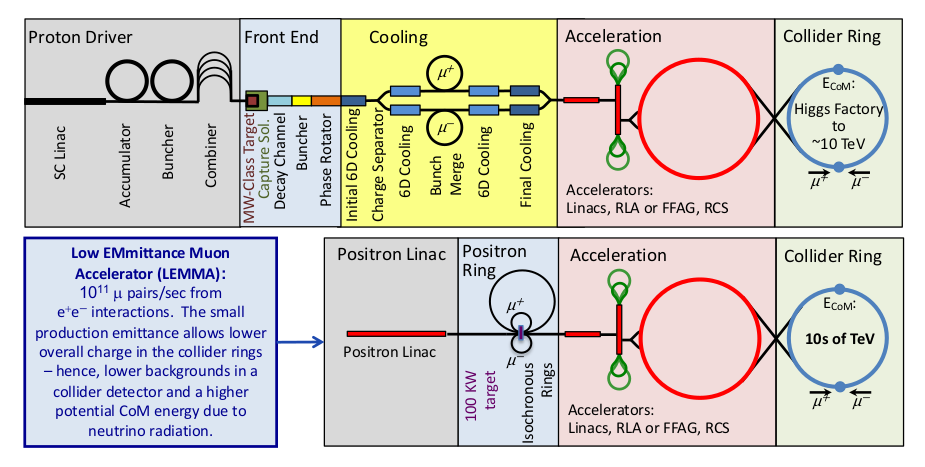
\includegraphics[width=13cm]{image/Ekran Görüntüsü - 2021-06-23 09-42-14.png}
\caption*{Şekil 4. Üst: protonlara dayalı bir müon kaynağı ile potansiyel bir müon çarpıştırıcısının şematik düzeni. Alt: pozitronlara dayalı bir müon kaynağı ile potansiyel bir müon çarpıştırıcısının şematik düzeni [5].}
	\end{figure}

İki ana müon çarpıştırıcı kavramı geliştirilmiş ve önerilmiştir: İlkinde müonlar, protonlar (Muon Accelerator Program) kullanılarak, ikincisinde ise pozitronlar (LEMMA) kullanılarak üretilir. Proton kaynaklı şema, pion bozunmasıyla klasik bir müon üretimine dayanmaktadır. MAP şemasının şematik bir düzeni Şekil 4'te gösterilmektedir. Yoğun bir proton demeti, daha fazla sayıda pion ürettiği bir hedefe gönderilir. Pionların bir kısmı, pozitif ve negatif yük işaretleri olan müon demetleri oluşturmak için yakalanan müonlara bozunur. Bu müon ışınlarının faz boşlukları üretim sürecinden dolayı çok büyüktür ve ömürleri müon bozunması nedeniyle sınırlıdır. 

\begin{figure}[h]
 \centering
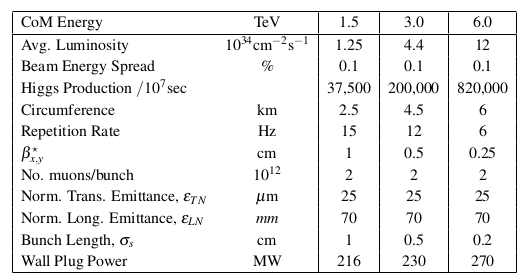
\includegraphics[width=10cm]{image/Ekran Görüntüsü - 2021-06-23 10-07-39.png}
\caption*{Tablo 1. MAP çalışmasından alınan bir müon çarpıştırıcısının temel parametreleri [5].}
	\end{figure}


 Pionların büyük bir kısmı, yakalanması ve soğutulması gereken müonlara bozunur. Müon İyonizasyon Soğutma Deneyi (MICE), 2019'da bu soğutmanın müon ömrü içinde elde edilebileceğini göstermişti. Bir soğutma sistemi, faz boşluklarını hızla azaltarak yüksek demet parlaklıklarına ulaşır.  Birkaç aşamada, demetler, müonların enerjisini kaybettiği, demet faz alanını azaltan ve ardından yeniden hızlandığı maddeye yönlendirilir. Demetler daha sonra son enerjiye doğru bir lineer ve halka kombinasyonunda hızlandırılır. Çarpıştırıcı halkasında müonlar bozunana kadar dolaşırlar. Bu tür bir çarpıştırıcının temel parametrelerinin örnekleri, farklı enerjiler için Tablo 1'de gösterilmektedir. MAP çalışması, küresel çarpıştırıcı parametrelerini ve yüksek manyetik alandaki RF boşlukları gibi birkaç önemli teknik konuyu ele almıştır. Tasarım seviyesine ulaşmamış olsa da, çarpıştırıcı parametrelerine güven vermek yeterince kapsamlıdır. Performans tahminini tam olarak doğrulamak için önemli bileşen ve demet testleri ve entegre bir tasarım gerekecektir [5,6].

Pozitron kaynaklı şemada, bir hedefte durgun durumdaki elektronlara çarpan 45 GeV pozitron, çok düşük bir emisyonla, reaksiyon eşiğine yakın müon çiftleri üretir. Bu nedenle, hiçbir müon demeti soğutması gerekli değildir ve demet akımı, aşağıda tartışılacağı gibi, MAP şemasındaki yüksek müon akımıyla ilgili bir dizi önemli zorluğu hafifleten MAP şemasındakinden çok daha küçük olabilir. Bununla birlikte, orijinal LEMMA tasarımının iki sorunu incelemede tanımlanmıştır, bu da ışınlılığı büyüklük sırasına göre potansiyel olarak azaltmaktadır. Şu anda, LEMMA ekibi bu sorunları çözmek için çarpıştırıcı konseptinin yeniden tasarlanmasını gerçekleştiriyor. Ancak, sonuçları değerlendirmek için henüz çok erken [5].

Diğer müon üretimi seçenekleri de araştırılabilir. Bir örnek, LEMMA şeması için potansiyel olarak pozitron üretimi için faydalı olabilecek bir \textit{ Gama Fabrikası}'nda düşük emisyonlu müon demetlerinin olası doğrudan üretimidir. Bu şemada, bir halkada depolanan kısmen yalınlaştırılmış ağır iyonlar, yoğun X ışınları patlamaları oluşturmak için bir lazer darbesi ile çarpışır [5].

\begin{figure}[h]
 \centering
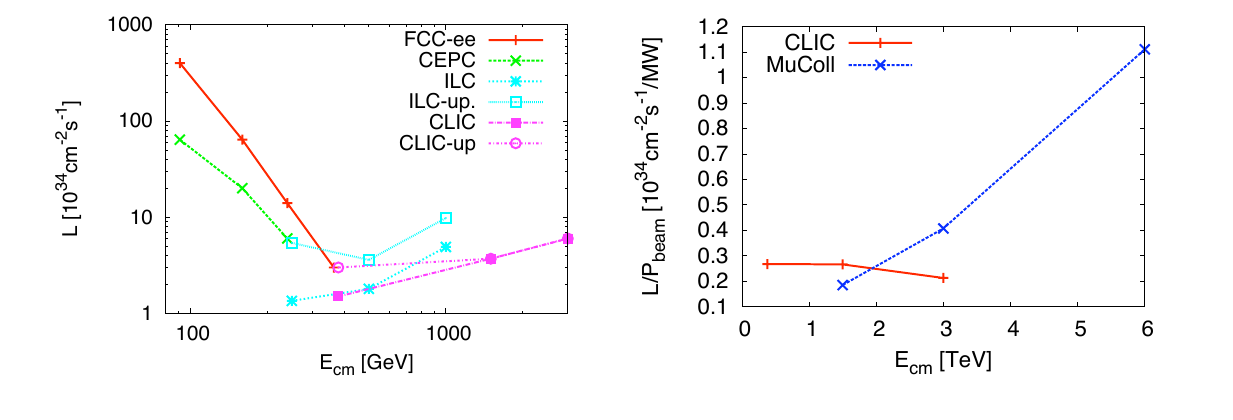
\includegraphics[width=17.5cm]{image/Ekran Görüntüsü - 2021-06-23 11-28-44.png}
\caption*{Şekil 5. Sol taraf: Granada'da sunulan FCC-ee, CEPC, ILC ve CLIC'in birleştiği tüm deneylerin ışınlıkları. Sağ taraf: CLIC ve proton tabanlı müon çarpıştırıcı şeması için kütle merkezi enerjisinin bir fonksiyonu olarak demet gücü başına IP (Interaction Point) başına ışınlık [5].}
	\end{figure}
	
	
\section{Yeni Fizik Potansiyeli}	

Lineer elektron-pozitron çarpıştırıcıları ile yüksek çarpışma enerjileri ve ışınlıkları elde edilebilir. Avrupa Parçacık Fiziği Stratejisi Güncellemesi çerçevesinde önerilen en yüksek kütle merkezi enerjisine CLIC tarafından $6 \times 10^{34} \textrm{ cm}^{-2} \textrm{ s}^{-1}$ ışınlılığı ile ulaşılabilmektedir. Bu öneri gelişmiş teknolojiye dayanmaktadır. Ancak, 3 TeV CLIC aşamasının entegre maliyeti yaklaşık 18 GCHF'dir ve güç tüketimi yaklaşık 590 MW'dir (28 MW demet gücü üretir). Tasarım maliyet ve güç açısından tam olarak optimize edilmemiştir ancak önemli değişiklikler beklenmemektedir. Bu nedenle, lineer çarpıştırıcıların uygun maliyetli kaynaklarla daha yüksek enerjilere ulaşabilecekleri açık değildir. 3 TeV enerji ölçeğinde bir müon çarpıştırıcısı CLIC ile rekabet edebilir. Tablo 1'deki güç tahmini, daha küçük bir tüketime işaret etmektedir. Yapılan maliyet çalışmaları, 6 TeV'lik bir müon çarpıştırıcısının 3 TeV'lik bir CLIC'den daha ucuz olabileceğini göstermektedir. Ancak sayıları doğrulamak veya düzeltmek için kavramsal bir tasarım gerekecektir. Müon çarpıştırıcısının sağlayabileceği potansiyel olarak önemli bir fayda, artan çarpışma enerjisi ile demet gücü başına ışınlıkta doğrusal bir artıştır. Buna karşılık lineer çarpıştırıcılarda demet gücü başına ışınlık doğal olarak çarpışma enerjisinden bağımsızdır. Şekil 5, CLIC'e kıyasla proton bazlı müon çarpıştırıcısı için demet gücü başına ışınlığın bağımlılığını göstermektedir.  Ayrıca müon çarpıştırıcısı birden fazla çarpışma noktasına hizmet edebilir. Işınlık spektrumu, güçlü bir şekilde azaltılmış sinkrotron radyasyonu ve ilk durum radyasyonu nedeniyle doğrusal bir elektron-pozitron çarpıştırıcısından büyük ölçüde daha iyi olabilir [5].

Müon çarpıştırıcısı, Higgs fabrikası Higgs bozonunu rezonans olarak üretebilir ve Higgs bozon kütlesinin etrafında onlarca MeV seviyesinde enerji taraması yapabilir. Bu ölçüm, Higgs bozonunun genişliğini ve Yukawa bağlaşımlarını doğrudan araştırabilir. Lepton çarpıştırıcılarının temiz ortamı, Higgs bozonunun birçok özel bozunması için hassas ölçümler de sağlar [7].

Ek olarak, müon bozunmaları, iyi bilinen bir akı ve enerji spektrumuna sahip elektron ve müon nötrinoları üreterek fiziğin başka bir önemli alanına katkı sağlar. Bu nötrinolar, Uzun Temel Hat Tesisleri için ideal tamamlayıcı oluşturacak olan bir Nötrino Fabrikası için kaynak görevi görebilir [1]. 

\section{Sonuçlar}

Bir müon çarpıştırıcısına sahip olmanın yeni fizik keşfi için birçok avantajı vardır. Bir müon çarpıştırıcısı, yüksek enerji fiziği için eşsiz bir lepton çarpıştırıcısı tesisi olacaktır. Bugün, müon çarpıştırıcısı kavramı FCC-ee, CLIC, ILC veya CEPC kadar eski değildir fakat en kısa zamanda müon çarpıştırıcısının fizibilitesini kanıtlamak, kalan önemli teknik zorlukları ele almak ve uygun fiyatlı ve kabul edilebilir bir güç tüketimine sahip kavramsal bir tasarım sağlamak için bir Ar-Ge programı oluşturulması çok önemlidir. Çok yüksek enerjili lepton sınırı için verilen sözler, bu fırsatın kaçırılmaması gerektiğini gösteriyor. Yeterli çaba gösterilebilirse, yaklaşık 25 yılda bir müon çarpıştırıcısı çalıştırmanın mümkün olacağı düşünülüyor. Mevcut temel yetkinliklerden yararlanmak ve bu zorlu projenin yol haritasını çizmek için iyi odaklanmış bir uluslararası çaba ise muhakkak gereklidir. Yeni teknolojilerin geliştirilmesi, diğer çarpıştırıcı projelerle sinerji içinde gerçekleşmesi fiziğin gelişimi için önemlidir. Ayrıca, yeni birçok deneylere de olanak sağlayabilir.



	\begin{thebibliography}{99}
	
	\bibitem{mano} Delahaye, J.P.; Diemoz, M.; Long, K.; Mansouli\'e, B.; Pastrone, N.; Rivkin, L.; Schulte, D.; Skrinsky, B.; Wulzer, A. (2019). \textit{Muon Colliders}. arXiv pre-print. arXiv:1901.06150.
	
	\bibitem{mano} Palmer, R.B. (2014). \textit{Muon Colliders}. Rev. Accel. Sci. Tech., 7, 137-159. doi:10.1142/S1793626814300072.
	
	\bibitem{mano} Schulte, D.; Pastrone, N.; Long, K. (2020). \textit{Sketching out a muon collider}. Erişim adresi: \url{https://www.cerncourier.com/a/sketching-out-a-muon-collider/}. Erişim tarihi: 22.06.2021.
	
	\bibitem{mano} Gray, H.M. (2021). \textit{Future colliders for the high-energy frontier}. Rev. in Physics, 6, 100053. doi:10.1016/j.revip.2021.100053.
	
	\bibitem{mano} Schulte, D.; Delahaye, J.P.; Diemoz, M.; Long, K.; Mansouli\'e, B. (2019). \textit{Muon Collider. A Path to the Future?} In European Physical Society Conference on High Energy Physics - EPS-HEP-19,Jul. doi:10.22323/1.364.0004.
	
	\bibitem{mano} MICE collaboration (2020). \textit{Demonstration of cooling by the Muon Ionization Cooling Experiment.} Nature 578, 53–59. doi:10.1038/s41586-020-1958-9.
	
	\bibitem{mano} Greco, M. (2016). \textit{Physics potential and motivations for a muon collider.} Int. Journal of Modern Phy. A, 31, 1630028. doi:10.1142/S0217751X16300283.


	\end{thebibliography}
	
\end{document}
